\chapter{Ocena aplikacji}
\label{cha:ocena}

W tym rozdziale zaprezentowana została kompleksowa ocena aplikacji \en. Jest ona
podzielona na kilka części. Następnie zaprezentowane są testy jakościowe, które
opierają się na próbie odzwierciedlenia wybranych zjawisk fizycznych przy pomocy
symulatora. Z kolei testy wydajnościowe wersji podstawowej oraz równoległej \en
pokazują zysk jaki dało przeniesienie obliczeń na kartę graficzną. Na podstawie
tych wyników zanalizowana została dostępność aplikacji dla potencjalnych
użytkowników na różnych urządzeniach oraz ich konfiguracjach. Rozdział kończy
ocena stopnia realizacji założeń projektowych oraz krótkie podsumowanie.

\section{Modelowanie wybranych zjawisk fizycznych jako testy jakościowe symulatora}

W przypadku aplikacji edukacyjnej jaką jest symulator \en niezwykle istotne jest
aby symulowane zjawiska odzwierciedlały w sposób  wiarygodny rzeczywistość. Z
drugiej jednak strony, aplikacja musi być interaktywna i działać w czasie
rzeczywistym. Dlatego też nie można sobie pozwolić na zbyt długi czas
wykonywania, co zwykle idzie w parze z dokładnymi algorytmami i obliczeniami. Z
tego też powodu zastosowane silniki (algorytmy) fizyczne balansują pomiędzy
poprawnością fizyczną, a wydajnością (por. rozdział \ref{sec:silnikiFizyczne}).
Jest to dopuszczalne, ponieważ symulacja jest zorientowana wyłącznie na aspekt
wizualny.

Z powodu tego kompromisowego podejścia do pełnej dokładności obliczeń, niezwykle
istotne były testy aplikacji pod kątem podstawowej poprawności fizycznej. W tym
celu zostały przygotowane przypadki testowe, które miały za zadanie modelować
powszechnie znane zjawiska fizyczne związane z przewodnictwem cieplnym oraz
dynamiką płynów. Poniżej przedstawione są wyniki tych testów.

\subsection{Komórki Bénarda}

Modelowanie komórek Bénarda to jeden z podstawowych testów aplikacji
symulujących dynamikę płynów. Są to komórki konwekcyjne powstające w płynie
podgrzewanym od spodu. Rysunek \ref{fig:physBenard} prezentuje wyniki symulacji
przeprowadzonej przez \en.

\begin{figure}[!h]
\centering
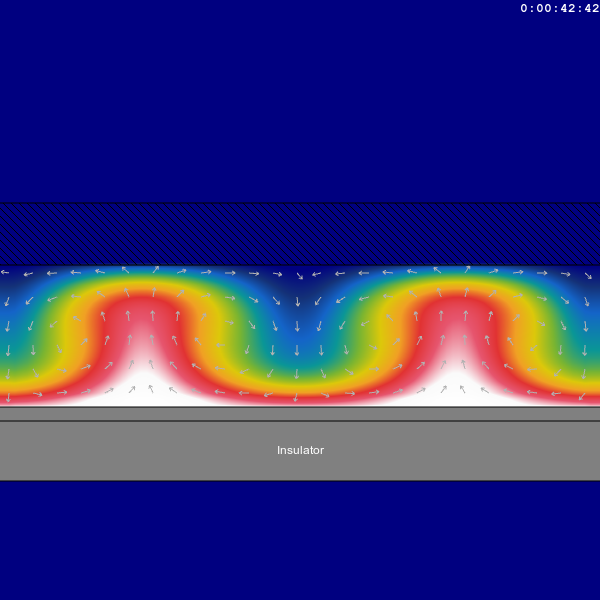
\includegraphics[width=0.8\textwidth]{img/physics/benard}
\caption{Symulacja formowania się komórek Bénarda}
\label{fig:physBenard}
\end{figure}

Wyraźnie widać formowanie się oczekiwanych komórek. Ich układ oraz kształt
stabilizuje się po bardzo krótkim czasie symulacji. Wyniki można uznać za w
pełni satysfakcjonujące.

\subsection{Przepływ laminarny oraz turbulentny}
\label{sec:przeplywyLamTur}

Symulacja przepływów laminarnych oraz turbulentnych to następny test silnika
dynamiki płynów. Rodzaj przepływu, w przypadku gdy jest on zakłócony przez
obecność przeszkody, w głównym stopniu determinuje liczba Reynoldsa. Jest ona
zależna od:

\begin{itemize}
\item lepkości płynu,
\item prędkości przepływu,
\item średnicy przeszkody.
\end{itemize}

W związku z tym został przygotowany przypadek testowy, w którym płyn ma stałą
lepkość, a przeszkody identyczne wymiary. Zmienna jest tylko prędkość przepływu.
Dla mniejszych prędkości oczekiwanym wynikiem był przepływ laminarny, dla
większych przepływ turbulentny. Rysunek \ref{fig:physLaminarTurbulent}
prezentuje wyniki takiej symulacji przeprowadzonej przez \en.

\begin{figure}[!h]
\centering
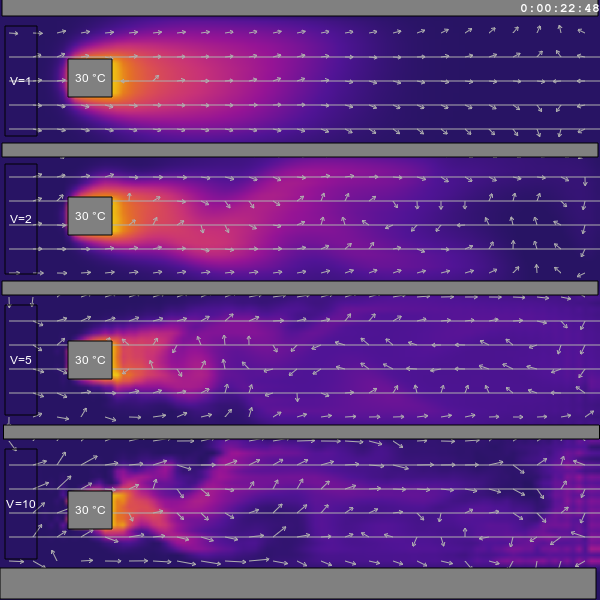
\includegraphics[width=0.8\textwidth]{img/physics/laminarTurbulent}
\caption{Symulacja wpływu liczby Reynoldsa na rodzaj przepływu}
\label{fig:physLaminarTurbulent}
\end{figure}

Rezultaty są zgodne z oczekiwaniami. Wyraźnie widać wpływ liczby Reynoldsa
(determinowanej przez prędkość płynu) na rodzaj przepływu.

\subsection{Ścieżka wirowa von Kármána}

Ścieżka wirowa von Kármána to kolejny doskonały test silnika dynamiki płynów.
Jest to szczególny rodzaj przepływu turbulentnego, który powstaje wyłącznie dla
pewnego zakresu wartości liczby Reyonldsa (por. \ref{sec:przeplywyLamTur}).

W związku z tym został przygotowany przypadek testowy, w którym płyn ma stałą
lepkość oraz prędkość przepływu, natomiast zmienna jest tylko średnica
przeszkody. Zgodnie z powyższymi założeniami, powinno być możliwe dobranie
takich średnic przeszkód, aby wiry Kármána powstały tylko za większą z nich.
Rysunek \ref{fig:physKarman} prezentuje wyniki takiej symulacji przeprowadzonej
przez \en.

\begin{figure}[!h]
\centering
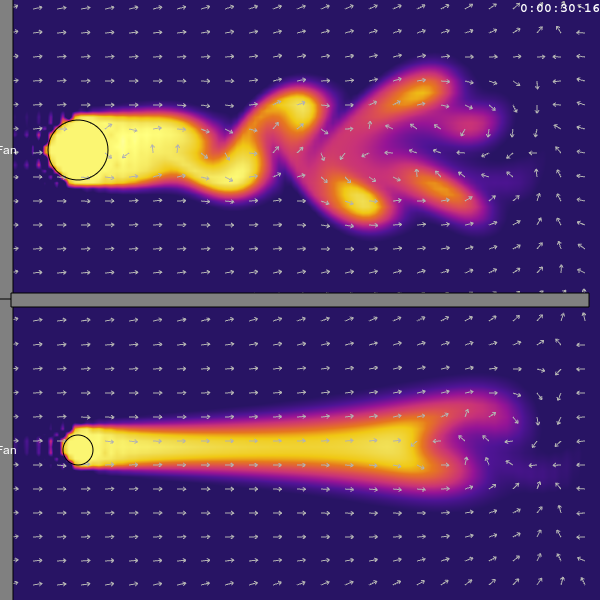
\includegraphics[width=0.8\textwidth]{img/physics/karman}
\caption{Symulacja formowania się wirów Kármána}
\label{fig:physKarman}
\end{figure}

Rezultaty są zgodne z oczekiwaniami. Wir powstał tylko w warunkach, w których
liczba Reynoldsa była większa.

\subsection{Pojemność cieplna}

Tym razem przypadek testowy dotyczy silnika przewodnictwa cieplnego. Pojemność
cieplna jest wielkość fizyczna, która charakteryzuje ilość ciepła, jaka jest
niezbędna do zmiany temperatury ciała o jednostkę temperatury. Poprawna
symulacja powinna uwzględniać ten parametr materiałów.

Aby to sprawdzić przygotowany został przypadek testowy, w którym znajdują się
dwa materiały o różnej pojemności cieplnej. Materiał o większej pojemności
powinien przewodzić ciepło znacznie lepiej niż ten o pojemności mniejszej.
Wyniki takiego eksperymentu przeprowadzonego przez symulator \en prezentuje
rysunek \ref{fig:heatCapacity}.

\begin{figure}[!h]
\centering
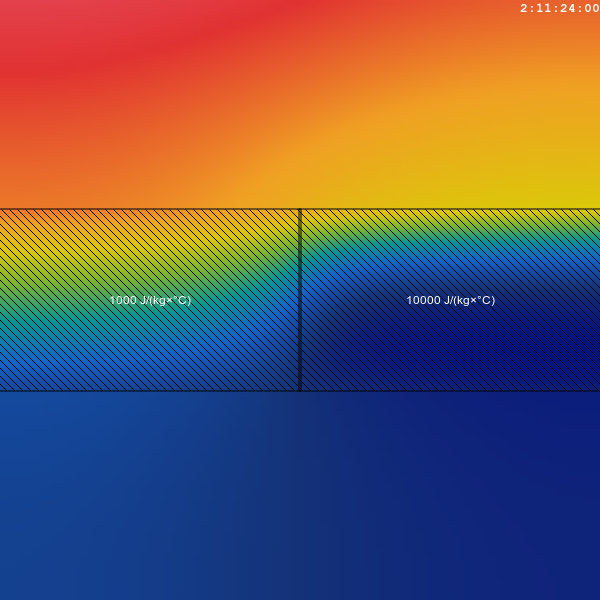
\includegraphics[width=0.8\textwidth]{img/physics/heatCapacity}
\caption{Symulacja wpływu pojemności cieplnej na przewodnictwo cieplne}
\label{fig:heatCapacity}
\end{figure}

Rezultaty po raz kolejny są zgodne z oczekiwaniami. Widać wyraźnie, iż materiał
o większej pojemności cieplnej znacznie lepiej przewodzi ciepło.

\subsection{Aspekt edukacyjny}

Ostatni z zaprezentowanych testów jest bardziej złożony. Nie prezentuje on
jednego, konkretnego zjawiska fizycznego jak poprzednie przykłady. Skupia się on
na zaprezentowaniu przykładowych możliwości symulacji oraz na potencjalnym
aspekcie edukacyjnym.

Przygotowana została scena zawierająca nieszczelnie izolowane pomieszczenie,
będące metaforą mieszkania. Jest ono ogrzewane przez element grzewczy o stałej
mocy. W jego otoczeniu został wymuszony dość mocny przepływ symulujący wiatr.
Miało to na celu pokazanie użytkownikom różnych, potencjalnych dróg ucieczki
ciepła z pomieszczeń mieszkalnych.

\begin{figure}[!h]
\centering
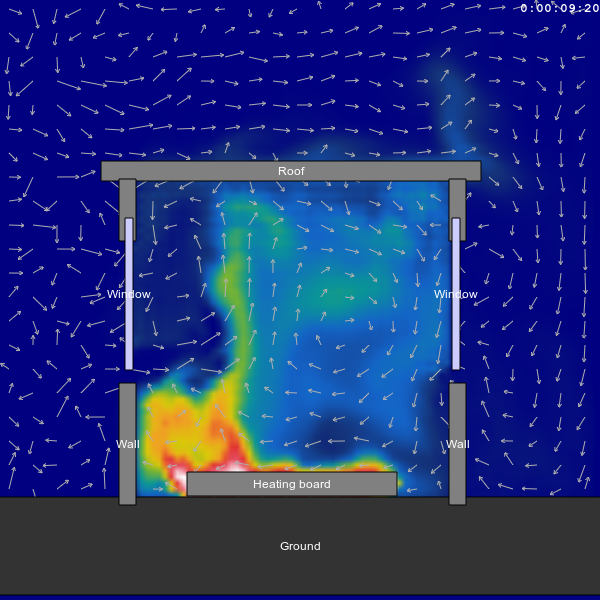
\includegraphics[width=0.8\textwidth]{img/physics/wind}
\caption{Symulacja ucieczki ciepła z pomieszczeń mieszkalnych}
\label{fig:wind}
\end{figure}

Rysunek \ref{fig:wind} prezentuje efekty takiej symulacji. Widoczne są dwa
wyraźne zjawiska -- strata ciepła w okolicy nieszczelnych okien oraz strata
ciepła związana z przewodnictwem cieplnym dachu. Pozwala to lepiej zrozumieć
użytkownikowi (docelowo uczniowi na początkowym etapie edukacji) wpływ różnych
aspektów pomieszczeń mieszkalnych (takich jak szczelność czy izolacja) na straty
ciepła. Może przyczynić się to do rozsądniejszego i ekonomiczniejszego
gospodarowania energią w jego własnym mieszkaniu czy też domu. W dobie
szczególnej dbałości o środowisko naturalne jest to niezwykle cenny i pożądany
efekt edukacyjny.

\section{Testy wydajnościowe}

Wydajność jest kluczowym aspektem symulacji ukierunkowanej na cele edukacyjne.
Tylko odpowiednia prędkość symulacji może przyciągnąć uwagę użytkownika i
zachęcić go do dalszej eksploracji zagadnienia.

W celu osiągnięcia zadowalającej wydajności na różnych urządzeniach zastosowano
kilka technik. Podstawową jest świadoma implementacja polegająca na unikaniu
zbędnych, czasochłonnych operacji, wynikająca ze znajomości środowiska
przeglądarki internetowej. Jednak krokiem, który najbardziej przyczynił się do
powstania naprawdę wydajnej aplikacji było przeniesienie obliczeń związanych
z fizyką na procesor karty graficznej.

Niniejsza sekcja przedstawia zyski z zastosowania tej optymalizacji. Omówiona
jest także kwestia wpływu konfiguracji sprzętowej użytkownika oraz związana z
tym ogólna dostępność symulatora dla szerokiego grona odbiorców.

\subsection{Metodologia testów}

Za wyznacznik wydajności została przyjęta liczba klatek na sekundę animacji,
którą jest w stanie generować działająca aplikacja \en. Jedna klatka domyślnie
składa się z:

\begin{itemize}
\item czterech kroków symulacji, 
\item odświeżenie wizualizacji.
\end{itemize}

Takie też ustawienia zostały zastosowane podczas wszystkich testów. 

Aplikacja wymusza kolejne klatki poprzez użycie metody \ow{setInterval()} z
czasem 0. Powoduje to, iż przeglądarka nie wprowadzi żadnych dodatkowych
opóźnień między klatkami i przejdzie do generowania kolejnej natychmiast, gdy
będzie to możliwe. Nie została użyta zalecana w przypadku aplikacji
\ow{WebGL}funkcja \ow{requestAnimationFrame()}, ponieważ wprowadza ona limit 60
klatek na sekundę i koncentruje się na utrzymaniu stałego tempa animacji, a nie
osiągnięciu maksymalnej wydajności. Zaburzało to w istotny sposób wiarygodność
wyników.

Na potrzeby testów zostały przygotowane specjalne przypadki testowe. Różnią się
one między sobą:
\begin{itemize} 
\item układem sceny, 
\item modelowanym zjawiskiem fizyczny,
\item użytymi silnikami fizycznymi:
	\begin{itemize} 
	\item wyłącznie silnik przewodnictwa cieplnego,
	\item silnik przewodnictwa cieplnego oraz silnik dynamiki płynów,
	\end{itemize}
\item rozmiarem siatki symulacyjnej.
\end{itemize}

Tabela \ref{tab:przypTest} prezentuje symboliczne nazwy przypadków testowych
wraz z ich krótką charakterystyką. Skrót HT pochodzi od ang. Heat Transfer i
oznacza, że dany przypadek testowy korzysta z silnika przewodnictwa cieplnego. Z
kolei skrót CDF pochodzi od ang. Computational Fluid Dynamics i oznacza, że dany
przypadek testowy korzysta z silnika dynamiki płynów. Wizualizację symulacji
przypadków testowych prezentują rysunki \ref{fig:ht1}, \ref{fig:ht2},
\ref{fig:cfd1} oraz \ref{fig:cfd2}.


\begin{table}
\caption{Zestawienie charakterystyki przypadków testowych do pomiaru wydajności}
\centering
\begin{tabular}{|l|c|c|c|l|}
\hline
nazwa testu & siatka & HT & CFD & opis \\ \hline
\textbf{ht1-100} & $100x100$ & \checkmark & $\times$ &
symulacja przewodnictwa cieplnego \\ \hline

\textbf{ht1-512} & $512x512$ & \checkmark & $\times$ &
symulacja przewodnictwa cieplnego \\ \hline

\textbf{ht1-1024} & $1024x1024$ & \checkmark & $\times$ &
symulacja przewodnictwa cieplnego \\ \hline

\textbf{ht2-100} & $100x100$ & \checkmark & $\times$ &
symulacja przewodnictwa cieplnego \\ \hline

\textbf{ht2-512} & $512x512$ & \checkmark & $\times$ &
symulacja przewodnictwa cieplnego \\ \hline

\textbf{ht2-1024} & $1024x1024$ & \checkmark & $\times$ &
symulacja przewodnictwa cieplnego \\ 

\hline \hline 

\textbf{cfd1-100} & $100x100$ & \checkmark & \checkmark &
symulacja dynamiki płynów \\ \hline

\textbf{cfd1-256} & $256x256$ & \checkmark & \checkmark &
symulacja dynamiki płynów \\ \hline

\textbf{cfd2-100} & $100x100$ & \checkmark & \checkmark &
symulacja dynamiki płynów \\ \hline

\textbf{cfd2-256} & $256x256$ & \checkmark & \checkmark &
symulacja dynamiki płynów \\ \hline
\end{tabular}

\label{tab:przypTest}
\end{table}

\begin{figure}[!p]
\begin{minipage}[b]{0.47\linewidth}
\centering
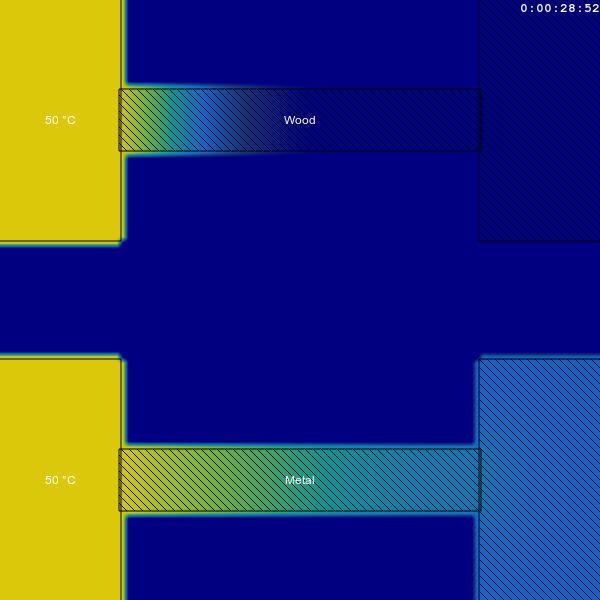
\includegraphics[width=\textwidth]{img/perfCase/ht1}
\caption{Symulacja ht1-100/512/1024}
\label{fig:ht1}
\end{minipage}
\hspace{0.04\linewidth}
\begin{minipage}[b]{0.47\linewidth}
\centering
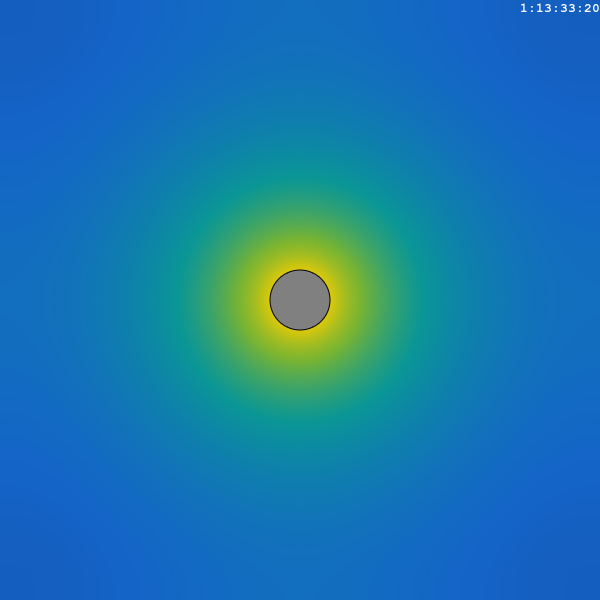
\includegraphics[width=\textwidth]{img/perfCase/ht2}
\caption{Symulacja ht2-100/512/1024}
\label{fig:ht2}
\end{minipage}
\end{figure}
\begin{figure}[!p]
\begin{minipage}[b]{0.47\linewidth}
\centering
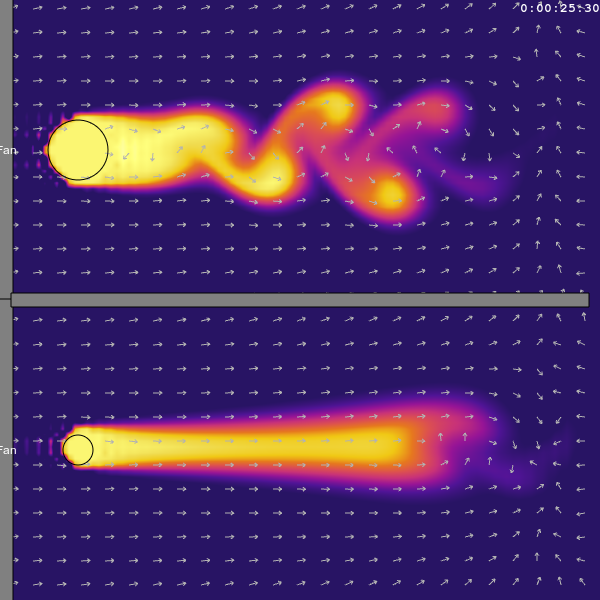
\includegraphics[width=\textwidth]{img/perfCase/cfd1}
\caption{Symulacja cfd1-100/256}
\label{fig:cfd1}
\end{minipage}
\hspace{0.04\linewidth}
\begin{minipage}[b]{0.47\linewidth}
\centering
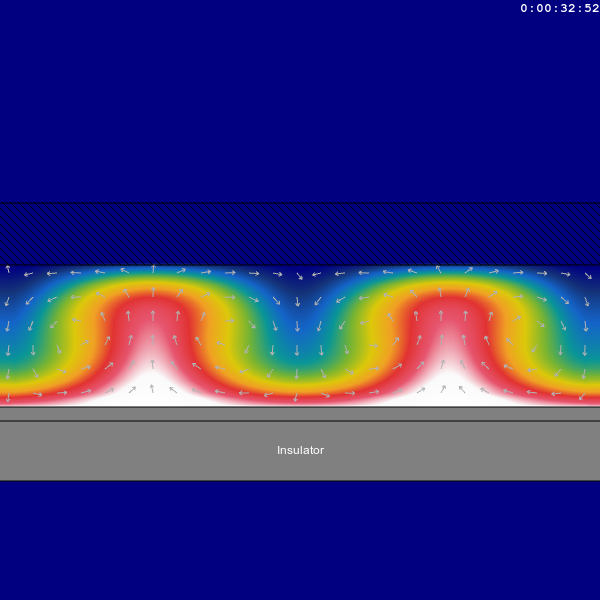
\includegraphics[width=\textwidth]{img/perfCase/cfd2}
\caption{Symulacja cfd2-100/256}
\label{fig:cfd2}
\end{minipage}
\end{figure}

\subsection{Konfiguracje sprzętowe przeznaczone do testów}

Testy zostały przeprowadzone na następujących komputerach:

\begin{itemize}

\item laptop Samsung QX510,
\item laptop Apple MacBook Pro, wersja z roku 2010,
\item laptop Apple MacBook Pro, wersja z roku 2012,
\item komputer stacjonarny.

\end{itemize}

\begin{table}[!h]
\caption{Charakterystyka komputerów testowych}
\centering
\begin{tabular}{|l|l|l|l|}
\hline
nazwa & procesor & karta graficzna & system operacyjny \\ \hline
Samsung QX510 & Intel Core i5 2.66GHz & NVIDIA GT 420M & Ubuntu 12.04 \\ \hline
MacBook Pro 2010 & Intel Core i7 2.66GHz & NVIDIA GT 330M & Mac OS X 10.6.8 \\ \hline
MacBook Pro 2012 & Intel Core i7 2.3GHz & NVIDIA GT 650M & Mac OS X 10.7.4 \\ \hline
stacjonarny & Intel Core2Quad 2.5GHz & NVIDIA 9600GT & Windows 7 \\ \hline
\end{tabular}
\label{tab:komputery}
\end{table}

Ich dokładną specyfikację prezentuje tabela \ref{tab:komputery}.
Konfiguracje znacznie różnią się od siebie. Działają pod kontrolą trzech
najpopularniejszych systemów operacyjnych -- Linux (Ubuntu), Mac OS X oraz
Windows 7. Również moc obliczeniowa kart graficznych jest bardzo zróżnicowana.

\subsection{Porównanie wydajności w różnych przeglądarkach internetowych}

Aplikacja od początku rozwoju była głównie testowana w przeglądarce Google
Chrome, gdyż wyraźnie było widać jej ogromną przewagę w kwestii wydajności
silnika \ow{JavaScript}. Ponadto, wg. ostatnich raportów, jest to
najpopularniejsza przeglądarka na świecie, tak więc potencjalnie najwięcej
użytkowników \en będzie z niej korzystać. Raport \cite{BrowserStats} pokazuję,
iż w lipcu 2012 roku z przeglądarki Google Chrome korzystało 42.9\% użytkowników
internetu. Drugie miejsce należało do przeglądarki Mozilla Firefox z udziałem
33.7\%. Łącznie te dwie przeglądarki posiadają 77.6\% ,,rynku'', dlatego są
traktowane priorytetowo. Kolejna popularna przeglądarka Internet Explorer
została wyłączona z testów z powodu niedostępności poza środowiskiem Windows
oraz braku wsparcia dla technologii \ow{WebGL}. Podobnie Safari, które wspiera
\ow{WebGL} jednak działa tylko na systemie operacyjnym Mac OS. Dlatego też testy
zostały przeprowadzone wyłącznie z użyciem następujących przeglądarek:

\begin{itemize}
\item Google Chrome v. 22
\item Mozilla Firefox v. 16
\item Opera v. 12.50
\end{itemize}

Środowiskiem testowym był laptop Samsung QX510 (por. tablica \ref{tab:komputery}).

\subsubsection{Obliczenia fizyczne wykonywane na CPU}

Wyniki pomiarów wydajności symulatora w przypadku obliczeń przeprowadzanych na
CPU prezentuje tabela \ref{tab:przegladarki} oraz wykres \ref{fig:browserPerf}.
Nietrudno dostrzec ogromną przewagę przeglądarki Google Chrome. Jest to efekt
zastosowanego w niej niezwykle wydajnego silnika \ow{JavaScript} o nazwie V8.
Opera oraz Mozilla Firefox posiadają zbliżoną wydajność, jednak Opera jest
nieznacznie szybsza. Warto też zauważyć, iż kiedy obliczenia fizyczne
przeprowadzane są na CPU, jedyną przeglądarką, która zapewnia odpowiednią
prędkość wykonywania się symulacji jest Google Chrome.

\begin{table}[!h]
\caption{Wydajność symulacji na CPU w zależności od przeglądarki}
\centering
\begin{tabular}{|c|p{3cm}|p{3cm}|p{3cm}|}
\hline
test & Google Chrome & Mozilla Firefox & Opera \\ \hline
ht1-100 & 45.20 & 11.12 & 11.83 \\ \hline
h1-512 & 3.24 & 0.45 & 0.98 \\ \hline
ht1-1024 & 0.92 & 0.11 & 0.25 \\ \hline
ht2-100 & 48.04 & 10.73 & 12.05 \\ \hline
ht2-512 & 3.34 & 0.40 & 0.84 \\ \hline
ht2-1024 & 0.89 & 0.11 & 0.22 \\ \hline
cfd1-100 & 22.25 & 2.51 & 3.84 \\ \hline
cfd1-256 & 4.24 & 0.38 & 0.93 \\ \hline
cfd2-100 & 20.60 & 2.35 & 4.58 \\ \hline
cfd2-256 & 3.71 & 0.30 & 0.73 \\ \hline
\end{tabular}
\label{tab:przegladarki}
\end{table}

\begin{figure}[!h]
\centering
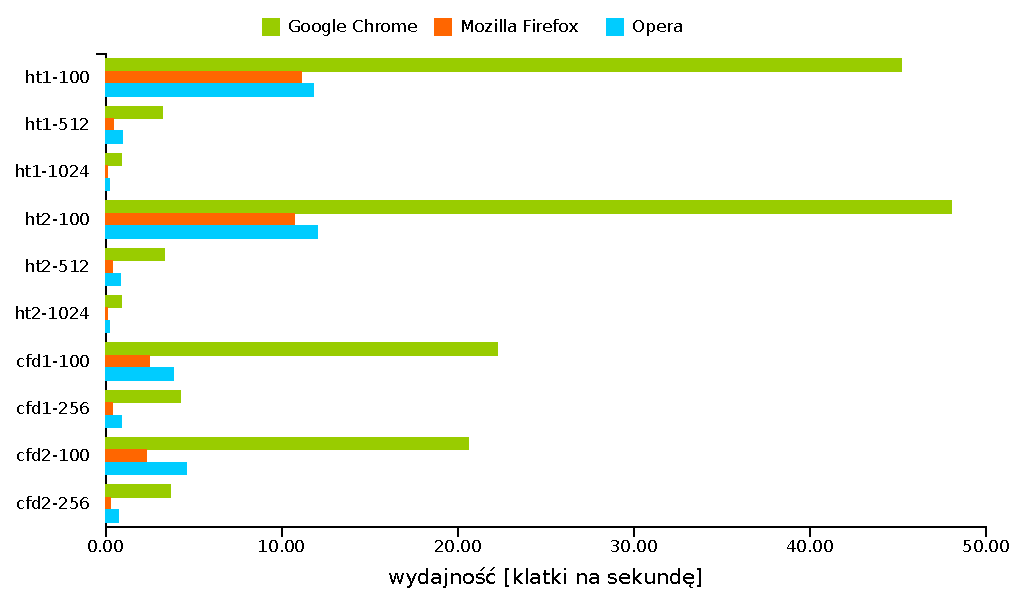
\includegraphics[width=\textwidth]{img/browserPerf}
\caption{Wydajność symulacji na CPU w zależności od przeglądarki}
\label{fig:browserPerf}
\end{figure}

\clearpage

\subsubsection{Obliczenia fizyczne wykonywane na GPU}

W przypadku symulacji, która obliczenia fizyczne przeprowadza na GPU, nie
została przetestowana Opera. Wynika to z faktu, iż w dniu kiedy testy były
przeprowadzane, wsparcie dla technologii \ow{WebGL} przez Operę nie było
wystarczające -- wyłącznie eksperymentalne w wyniku czego nie było
dostępu do niezbędnego rozszerzenia \ow{OES\_texture\_float}. Wyniki testów dla
przeglądarek Google Chrome oraz Mozilla Firefox przedstawiają tabela
\ref{tab:przegladarkiGPU} oraz wykres \ref{fig:browserPerfGPU}.

\begin{table}[!h]
\caption{Wydajność symulacji na GPU w zależności od przeglądarki}
\centering
\begin{tabular}{|c|p{3cm}|p{3cm}|}
\hline
test & Google Chrome & Mozilla Firefox \\ \hline
ht1-100 & 51.57 & 37.33 \\ \hline
h1-512 & 12.94 & 12.99 \\ \hline
ht1-1024 & 3.73 & 3.64 \\ \hline
ht2-100 & 48.84 & 37.59 \\ \hline
ht2-512 & 12.52 & 12.28 \\ \hline
ht2-1024 & 3.60 & 3.47 \\ \hline
cfd1-100 & 36.67 & 30.59 \\ \hline
cfd1-256 & 13.47 & 12.35 \\ \hline
cfd2-100 & 33.28 & 31.01 \\ \hline
cfd2-256 & 10.85 & 11.18 \\ \hline
\end{tabular}
\label{tab:przegladarkiGPU}
\end{table}

\begin{figure}[!h]
\centering
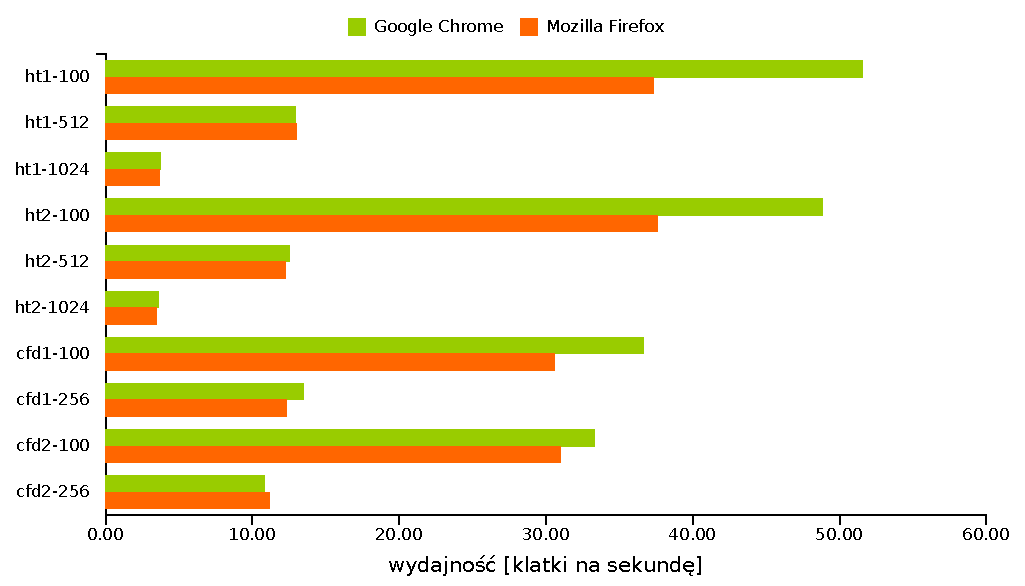
\includegraphics[width=0.9\textwidth]{img/browserPerfGPU}
\caption{Wydajność symulacji na GPU w zależności od przeglądarki}
\label{fig:browserPerfGPU}
\end{figure}

\clearpage

W przypadku obliczeń na GPU sytuacja diametralnie się zmienia. Różnice między
przeglądarkami, tak istotne przy obliczeniach na CPU, stają się znikome. Wynika
to z faktu, iż najbardziej obciążające obliczenia przeniesione są na kartę
graficzną i to jej wydajność jest decydująca, a nie wydajność silnika
\ow{JavaScript}. Potwierdza to fakt, iż przewagę Google Chrome widać wyłącznie
dla testów działających na najmniejszych siatkach. Są to jedyne przypadki, 
gdzie wydajność samego interpretera \ow{JavaScript} jest jeszcze istotna.

Innym ważnym wnioskiem jest to, iż użycie technologii \ow{WebGL} pozwala 
zniwelować różnice między wydjnością przeglądarek. O ile w przypadku obliczeń
na CPU jedynym rozsądnym środowiskiem wykonywania się symulacji była przeglądarka
Google Chrome, to przy zastosowaniu \ow{WebGL} możliwe staje się również użycie
Mozilli Firefox oraz każdej innej przeglądarki, która wspiera \ow{WebGL} (np.
Safari czy też w niedalekiej przyszłości także Opery).

\subsection{Analiza zysku wydajności wynikający z przeniesienia obliczeń na GPU}

\subsection{Wpływ optymalizacji i równoległości na jakość symulacji}

[TODO: rysunki, omówienie problemów z dokładniejszą siatką]

\section{Ocena dostępności aplikacji dla potencjalnych użytkowników}

\subsection{Wpływ posiadanej konfiguracji sprzętowej i oprogramowania na
symulator}

\section{Realizacja kluczowych wymagań}

\section{Podsumowanie}
